\section{Locus of the Incenter in a Generic Pair}
\label{sec:07-proof-theorem}

Recall the locus of the incenter and excenters are ellipses if the pair is confocal, see \cref{thm:02-incenter-excenter}. Here we expand the analysis, starting with the circumcircle family. The techniques developed here will help us expand the result to any generic pair.

\begin{proposition}
\label{prop:07-X1c}
Over Poncelet 3-periodics in the pair with an outer circle and an ellipse in generic position, the locus $X_1$ is given by:
\begin{align*}
  X_1:&\;z^4 - 2(( \bar{f} + \bar{g}) \lambda +  f g) z^2 + 8   \lambda z\\
  &+ (\bar{f} - \bar{g})^2 \lambda^2 +2 (  |f|^2 g +   f |g|^2 - 2 f - 2 g) \lambda + f^2 g^2=0\\
  \;&:\;  z^4 - 2\beta  z^2+ 8\lambda z+  (\beta^2-4\alpha\lambda) =0
\end{align*}
\end{proposition}

%\textcolor{red}{ronaldo pode mudar $a$,$b$,$c$ em $z_{12}$ etc?}
%\textcolor{blue}{ so agora vi. Olhei no pdf e nao olhei no texto. VOu tentar simplificar.}
%\textcolor{red}{mark tb sugeriu q vc olhe a prop 3.5 neste \href{https://studymath.github.io/assets/docs/real_complex_bash.pdf
%}{pdf}}

\begin{proof} The incenter of a triangle with vertices $\{z_1,z_2,z_3\}$ is given by:
\begin{align*}
    X_1&=\frac{\sqrt{s_1}\;z_1+\sqrt{s_2}\;z_2+\sqrt{s_3}\;z_3}{\sqrt{s_1}+\sqrt{s_2}+\sqrt{s_3}}\\
    s_1&=|z_2-z_3|^2, \; s_2=|z_1-z_3|^2, \;\; s_3=|z_2-z_1|^2
 % X_1=-\sqrt{z_1 z_2}-\sqrt{z_1z_3}-\sqrt{z_2z_3}
\end{align*}
 Using that $z_i\in \T$ it follows that
 \[s_1=2-(\frac{z_3}{z_2}+\frac{z_2}{z_2}),\;\; s_2=2-(\frac{z_1}{z_3}+\frac{z_3}{z_1}),\;\;s_3=2-(\frac{z_1}{z_2}+\frac{z_2}{z_1})\]
Eliminating the square roots in  the equation $X_1-z=0$ and using the relations  $\sigma_i$ (i=1,2,3) given in Blaschke's parametrization the result follows.
\end{proof}

\begin{remark} For $z_i\in \T^1$ we have  that $ X_1: -\sqrt{z_1 z_2}-\sqrt{z_1z_3}-\sqrt{z_2z_3}$. See \ref{exe:05-X1}
\end{remark} 

Using the same techniques in the last proof we can derive the locus of the incenter for 3-periodics in any ellipse pair:

 \begin{proposition}
\label{prop:07-X1g}
Over Poncelet 3-periodics in a generic nested ellipse pair, the locus of $X_1$ and the excenters is given by the roots of the following quartic polynomial in $z$:

 {\small
\begin{align*}
X_1&: \;\; ( p^2-q^2 )^{2}  {\lambda}^{2}{z}^{4}-4
\,\lambda\,p q (  ( {\lambda}^{2}+\beta ) {p}^{2}-
 ( 2\,\alpha\,\lambda+2 ) p q+ ( {\lambda}^{2}+\beta
 ) {q}^{2} ) {z}^{3}\\
 &+ ( -2\,\beta\,{\lambda}^{2}{p}^{
4}+2\,\lambda\, ( 2\,\alpha\,{\lambda}^{2}+\alpha\,\beta+9\,
\lambda )  {p}^{3} q+ ( -4\,{\alpha}^{2}{\lambda}^{2}-8\,
\beta\,{\lambda}^{2}-20\,\alpha\,\lambda+4\,{\beta}^{2}) {p}^{2} {q}^{2
} \\
&+2\,\lambda\, ( 2\,\alpha\,{\lambda}^{2}+\alpha\,\beta+9
\,\lambda ) p {q}^{3}-2\,\beta\,{\lambda}^{2}{q}^{4} ) {z}^
{2} 
 + ( 8\,{\lambda}^{3}{p}^{4}-4\,\lambda\, ( \beta\,{
\lambda}^{2}+6\,\alpha\,\lambda-{\beta}^{2} ) {p}^{3} q\\
&+ ( 4
\,\alpha\,\beta\,{\lambda}^{2}+16\,{\alpha}^{2}\lambda-4\,{\beta}^{2}
\alpha+20\,{\lambda}^{3}-4\,\beta\,\lambda ) {p}^{2}{q}^{2}-4\,
\lambda\, ( \beta\,{\lambda}^{2}+6\,\alpha\,\lambda-{\beta}^{2}
 ) p {q}^{3}\\
 &+8\,{\lambda}^{3}{q}^{4} ) X-{\lambda}^{2}
 ( 4\,\alpha\,\lambda-{\beta}^{2} ) {p}^{4}+2\,\lambda\,
 ( 4\,{\alpha}^{2}\lambda-{\beta}^{2}\alpha+2\,{\lambda}^{3}-
\beta\,\lambda )  {p}^{3} q \\
&+ ( -4\,{\alpha}^{3}\lambda+{
\alpha}^{2}{\beta}^{2}-12\,\alpha\,{\lambda}^{3}+2\,{\beta}^{2}{
\lambda}^{2}+2\,\alpha\,\beta\,\lambda+{\lambda}^{2} ) {p
}^{2}{q}^{2}\\
&+2\,\lambda\, ( 4\,{\alpha}^{2}\lambda-{\beta}^{2}\alpha+2\,
{\lambda}^{3}-\beta\,\lambda ) p {q}^{3} -{\lambda}^{2} ( 4\,
\alpha\,\lambda-{\beta}^{2} ) {q}^{4}
\end{align*}
}

\end{proposition}

\begin{proof} Let $p,q\in \mathbb{R}$. Consider the affine transformation
$T(z)=pz+q\ol z$ and set $w_i=T(z_i)$. The proof is similar to that given in \cref{prop:07-X1c}.  Here, in order  to simplify the vertices $z_i$ it is necessary to evaluate the sums
$p_k=z_1^k+z_2^k+z_3^k$ $(k=1,\ldots, 5)$, expressing the result in terms of $\alpha$, $\beta$ and $\lambda$. See \cref{fig:07-tafim}
\end{proof}
\begin{figure}
    \centering
    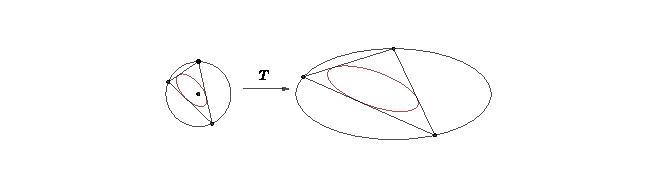
\includegraphics[width=1.0\textwidth]{pics_07_070_Tafim_par_elipses.pdf}
    \caption{Affine image of pair of a Poncelet pair with outer unitary circle having 3-periodics.  }
    \label{fig:07-tafim}
\end{figure}

%\textcolor{red}{ronaldo: organiza, %eu chamaria $p_1$ e $p_2$ talvez %de $X_1$ e de $[e_1,e_2,e_3]$, %mexer no exercicio.}

The above entails yet another alternative proof for the ellipticity of the $X_1$ locus over billiard 3-periodics:

\begin{corollary}
Over billiard 3-periodics, the locus of $X_1$ is given by:
%\[2\,ab{\lambda}^{2}{z}^{2}+2\,\lambda\, \left( {a}^{3}{\lambda}^{2}-{b}
%^{3}{\lambda}^{2}-{a}^{3}-{b}^{3} \right) z+{c}^{2} \left( {c}^{2}{
%\lambda}^{4}-2\,ab{\lambda}^{2}-{c}^{2} \right)=0 \]
 \[   X_1 =z-{\frac { \left( -{a}^{4}+{b}^{4}+{c}^{2}\delta \right) \lambda}{2\,{a
}^{2}{b}^{2}}} -\frac{    ( a^2 + b^2)\delta -a^4 - b^4}{ 2 a^2 b^2 \lambda}=0
\]
%$-\frac{    ( a^2 + b^2)\delta -a^4 - b^4}{ 2 a^2 b^2 \lambda}$
\label{cor:07-X1q2} 
\end{corollary}

\begin{proof}
Let $a$ and $b$ be the semi-axes of the billiard. In the confocal pair 
we have that
\[f={\frac {1}{c}\sqrt { 2\,\delta-{a}^{2}-{b}^{2}}}, \;\; g= -{\frac {1}{c}\sqrt {2\,\delta-{a}^{2}-{b}^{2} }}\]
This is obtained by taking an affine map
$T(z)=(a+b)z/2+(a-b)\bar{z}/2$ sending the pair with an unitary outer circle to the confocal pair, see   \cref{sec:02-caustic}.  

The result follows by factorization of the quartic  polynomial that defines $X_1$ in \cref{prop:07-X1g}.

Using CAS we obtain that $X_1$ is factorizable as $E_1 E_2$, where
{\small  
\begin{align*}
    E_1&=z-{\frac { \left( -{a}^{4}+{b}^{4}+{c}^{2}\delta \right) \lambda}{2\,{a
}^{2}{b}^{2}}} -\frac{    ( a^2 + b^2)\delta -a^4 - b^4}{ 2 a^2 b^2 \lambda}=0
%
\\
    E_2&= -2c^2\lambda\left[-2\,{a}^{2}{b}^{2}\lambda\,{z}^{3}+ \left(  \left( {c}^{2}{\lambda}^{2
}-{a}^{2}-{b}^{2} \right) \delta+{c}^{2} \left( {a}^{2}+{b}^{2}
 \right) {\lambda}^{2}-{a}^{4}+4\,{a}^{2}{b}^{2}-{b}^{4} \right) {z}^{
2}\right.
\\
& \left.   -4\,\lambda\,{c}^{2} \left( {a}^{2}+{b}^{2}+\delta \right) z-4\,{
\lambda}^{2} \left( {a}^{4}+{b}^{4}+{a}^{2}\delta+{b}^{2}\delta
 \right) 
\right]
\end{align*}
}
\end{proof}

\begin{corollary}
The locus $X_1$ is the ellipse with semi-axes given by $a_1=(a^2-\delta)/b$ and $b_1=(\delta-b^2)/a.$

%\[z= {\frac { \left( a-b \right)  \left(\delta -{a}^{2}-ab-{b}^{2}
 %\right) \lambda}{2\,ab}}-{\frac { \left( a+b %\right)  \left(  \delta-{a}^{2}
%+ab-{b}^{2} \right) }{2\,ab\lambda}}\]
 
\end{corollary}

\begin{proof}
Follows directly from  \cref{lem:ell-param} and  \cref{prop:07-X1q2}.
\end{proof}

\begin{remark}
The space of possible choices of two conics which admits a 3-periodic family is five dimensional.
\end{remark}

This stems from the fact that a conic has five degrees of freedom, so two conics have 10; the euclidean transformation group is 4-dimensional, and Cayley deducts one degree of freedom. Therefore: 10-4-1=5.

Note that over said 5d space, the possible confocal configurations are 1-dimensional. Interestingly, experimental evidence suggests that our very first result (elliptic locus of the incenter and excenters) is actually very rare:

\begin{conjecture}
Over Poncelet 3-periodics in a given pair of conics, the locus of the incenter and excenters are ellipses if and only if the pair is confocal.
\label{conj:07-incenter-excenter-loci}
\end{conjecture}

%Evidence also suggests:
%\textcolor{red}{ronaldo is this correct? da uma olhada nos \href{https://bernard-gibert.pagesperso-orange.fr/Tables/table28.html}{strong and weak points do gibert} -- mark sugere investigar se a conjectura certa é nao-racional nos sidelenghts squared}

%\begin{conjecture}
%If a given triangle center $X_k$ has trilinear (or barycentric) coordinates which are irrational on the sidelengths, then the locus of $X_k$ is non-elliptic.
%\end{conjecture}
